\documentclass{report}

\usepackage{enumerate,fullpage,graphicx,hyperref}

\title{Emergent Architertural Design}
\date{Last edited: \today}
\author{Project members: \\
	Derk-Jan Karrenbeld - 4021967\\
	Joost Verdoorn - 1545396\\
	Steffan Sluis - 4088816\\
	Tung Phan - 4004868\\
	Vincent Robbemond - 4174097
	}

\begin{document}
	\maketitle

	\pdfbookmark{\contentsname}{toc}
	\tableofcontents

	\clearpage

	\setcounter{section}{0}
	\renewcommand*\thesection{\arabic{section}}
	
	\section*{Introduction}
		This document contains the architectural design for the application created during the Context Project `Programming Life: Synthetic Biology'. The design is explained first in terms of a subsystem decomposition, which serves to uncover the inner workings of the application. Secondly, a description of the communication between the client and server is given, seeing as it is a key part of the application. Lastly, a short summary of the application architecture is given.
	\clearpage
	\section{Subsystem Decomposition}
		This section describes the key subsystems in the application. It is divided into two sections, one about the server-side subsystems and one about the client-side subsystems. The link between these two components will be discussed in the next section.
		\subsection{Server side}
			The server subsystems consist of two key parts: the server backend and the database. The server backend isn't used very much until the application is very nearly finished. It's main use is synchronisation between different client-backends and it could possibly be used to do calculations that are too complicated for the client-side of the application.\\
			The database is used for storage of user data, modules for cell design, as well as cell models created using the application. It provides a centralized storage so the client-side application can function on any platform without first having to tranfer any user data.
		\subsection{Client side}
			The client side subsystems contain most of the applications functionality. These subsystems are responsible for displaying the graphical environment with all it's modules, as well as doing the basic simulating. If the simulation becomes too complex, the complicated calculations can be sent to the sever to be processed on the server side. 
	\clearpage
	\section{Communication between client and server}
		The communication between client and server is a key aspect of the application. The communication done using \emph{REST} and \emph{AJAX}. This entails that the server waits for a request from the client, thus the client controls all communication. Combined with the fact that the server serves mostly to centralize the data storage and complicated calculations, this makes it so the client side of the application can be very resource efficient, so as to work on any platform.\\
		The image below shows a high level view of the different components and the tools used for constructing them:\\
		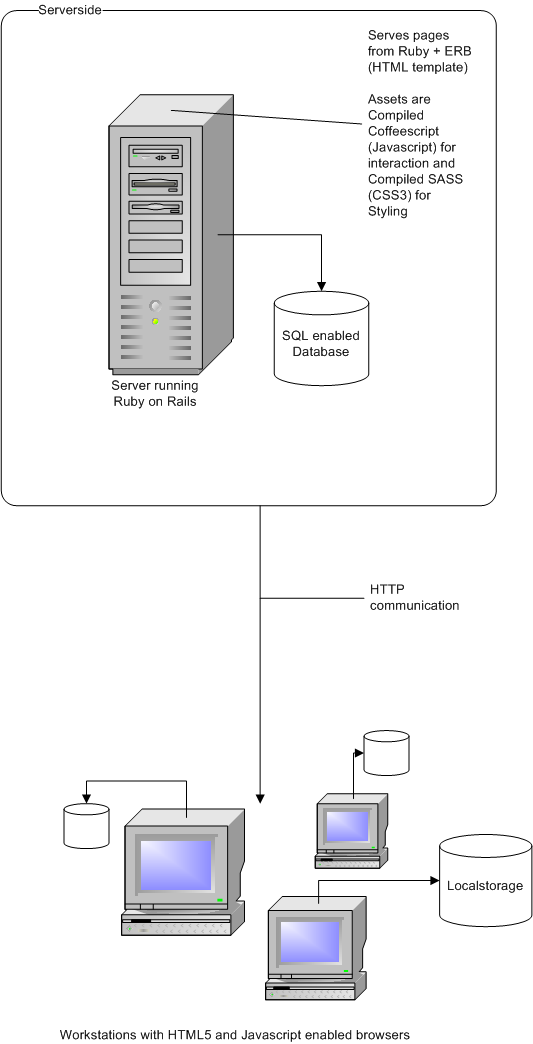
\includegraphics[width=16cm]{EAD.png}
	\clearpage
	\section{Summary}
		The application is a lightweight, cross-platform graphical design tool with a centralized storage database. The architecture ensures it's functionality on different kinds of machines as well as the ease of simulating complex cell models.
\end{document}
